%% Be sure to check spelling!

\documentclass{article}
\usepackage{amsmath}
\usepackage{epsfig}
\usepackage{listings}
\usepackage[letterpaper, margin=0.75in]{geometry}
\usepackage{EGR103F19}
\usepackage{fixltx2e}
\begin{document}

\begin{center}
\rule{6.5in}{0.5mm}\\~\\
\textbf{\large EGR 103L -- Fall 2019}\\~\\
\textbf{\huge \LaTeX~Assignment}\\~\\
Marcus Deans (md374)\\ 
Lab Section 2, Tuesdays 11:45-14:35\\
Due 8 September 2019\\~\\
{\small I understand and have adhered to all the tenets of the Duke
  Community Standard in completing every part of this assignment.  I
  understand that a violation of any part of the Standard on any part
  of this assignment can result in failure of this assignment, failure
  of this course, and/or suspension from Duke University.} 
\rule{6.5in}{0.5mm}\\
\end{center}

\tableofcontents
\listoffigures
\pagebreak

\section{Equations} %%% You will add your equations here
\begin{itemize}
\item General second-order system equation\cite[p.~221]{Rizzoni}:
% unnumbered and aligned equation
\begin{align*}
\frac{1}{\omega^2_n}\frac{d^2x(t)}{dt^2}+\frac{2\zeta}{\omega_n}\frac{dx(t)}{dt}+x(t)=K_Sf(t)
\end{align*}
\item The Secant Formula for finding maximum stress 
in a column\cite[p.~681]{Hibbeler}:
% unnumbered and aligned equation
\begin{align*}
\sigma_\mathrm{{max}}= \frac{P}{A}\left[1+\frac{ec}{r^2}\mathrm{sec}\left(\frac{L}{2r}\sqrt\frac{P}{EA}\right)\right]
\end{align*}
\item Characteristic determinant for a 2x2 system of 
differential equations\cite[p.~152]{Kreyszig}:
% aligned numbered equations...except no numbers on first parts
\begin{align}
\mathrm{det} \left(\mathrm{\textbf{A}}-\lambda\mathrm{\textbf{I}}\right)&=\nonumber
\begin{array}{|cc|}
a_{11}-\lambda & a_{12}\\
a_{21} & a_{22}-\lambda
\end{array}\\
&= \left(a_{11}-\lambda\right)\left(a_{22}-\lambda\right)-a_{12}a_{21}\nonumber\\
&= \lambda^2-\left(a_{11}+a_{22}\right)\lambda+a_{11}a_{22}-a_{12}a_{21} = 0
\end{align}
\item Definition of the Lyapunov exponent\cite[p.~56]{Ott}:
% aligned numbered equations
\begin{align}
h&= \lim_{T\to\infty}\frac{1}{T}\ln\left|\frac{\mathrm{d}x_T}{\mathrm{d}x_0}\right| \\
h&= \lim_{T\to\infty}\frac{1}{T}\sum_{n=0}^{T-1}\ln\left|M'\left(x_n\right)\right| \\
h&= \int\ln\left|M'\left(x\right)\right|d\mu\left(x\right)
\end{align}
\end{itemize}


\section{Tables using \texttt{tabular} and \texttt{array}}
\subsection{Using \texttt{tabular}} %%% You will add the tabular here
Converting ammonia into nitric acid - the Ostwald Process\cite{Ostwald}:
\begin{center}
\begin{tabular}{r|l}
Description & Chemical equation\\ \hline
Oxidization of Ammonia & 4 NH$\textsubscript{3}$ (g) + 5 O$\textsubscript{2}$ (g)
$\rightarrow$ 4 NO (g) + 6 H$\textsubscript{2}$O (g)\\
Oxidization of Nitric Oxide & 2 NO (g) + O$\textsubscript{2}$ (g)
$\rightarrow$ 2 NO$\textsubscript{2}$ (g)\\
Absorption of Nitrogen Dioxide & 3 NO$\textsubscript{2}$ (g) + H$\textsubscript{2}$O (l) $\rightarrow$ 2 HNO$\textsubscript{3}$ (aq) + NO (g)\\
\end{tabular}
\end{center}
% centered tabular here
\subsection{Using \texttt{array}} %%% You will add the array here
% stretched array here
\renewcommand{\arraystretch}{1.5}
\begin{center}
\[
\begin{array}{|c|c|}\hline
\mathrm{Equation} & \mathrm{ Description}\\ \hline \hline
\vec{v}=v_x\hat{i}+v_y\hat{j}+v_z\hat{k} & \mbox{Resolution }\mbox{into }\mbox{components}\\ \hline
v^2 = v_0^2 + 2a\Delta x & \mbox{Velocity }\mbox{formula}\\ \hline
\end{array}
\]
\end{center}
\pagebreak

\section{Comments} %%% You will add your comments here
Things I learned in this assignment:
% itemized list here
\begin{itemize}
\item How to use the \texttt{align} and \texttt{align*} environment to typeset numbered and unnumbered equation and using the nonumber command to suppress numbering equations in an align environment:
\item How to use \$ to enter math mode in a line of text to type shorter mathematical expression like $10^6$ and $\nabla u$ or Greek letters like $\Delta$;
\item How to use the \texttt{mathrm} command to put super- and subscripts in regular, versus italic, type for things like $V_{\mathrm{min}}$ instead of $V_{min}$;
\item How to change the appearance of fonts to make word \textbf{bold}, \textit{italics}, \underline{underlined}, or \texttt{typewriter font};
\item How to use \LaTeX~  in general!
\item How to use more complex math symbols and terms like summation and integrals, etc.
\item Using the tabular format
\item Learning how to use the array in two different forms, both within a series of equations as well as on its own in a table-like format.
\item Troubleshooting for problems like specific formatting (subscripts) 
\end{itemize}
\pagebreak
\appendix
\section{Codes}
%%% Everything in this section is done; make sure you 
%%% understand how it works in general
\lstset{style=python103, language=python} 
% above changes all listings to python style from EGR103S19
\subsection{Listing of full sample header for original code}
\lstinputlisting{Header1f.py}
\subsection{Listing of short sample header for original code}
\lstinputlisting{Header1s.py}
\subsection{Listing of full sample header for modified code}
\lstinputlisting{Header2f.py}
\subsection{Listing of short sample header for modified code}
\lstinputlisting{Header2s.py}
\pagebreak
\subsection{Listing code for sample graph on following page}
\lstinputlisting[language=Python]{MakeSample.py}

\pagebreak
\section{Figures \label{FigureList}}
%%% Everything in this section is done; make sure you 
%%% understand how it works in general

\begin{figure}[htb]
\begin{center}
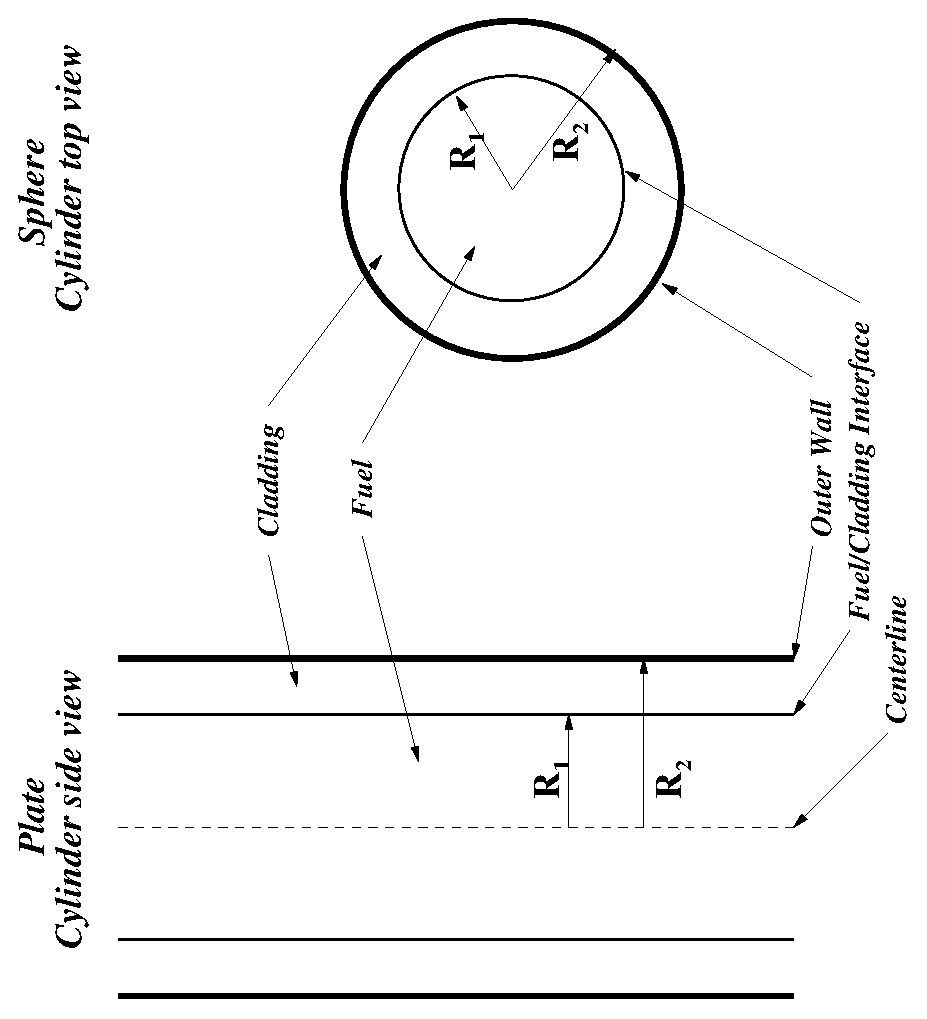
\epsfig{file=drawing.eps, width=3in, angle=-90} 
\caption{Drawing from ME 431L test.}
\end{center}
\end{figure}

\begin{figure}[htb]
\begin{center}
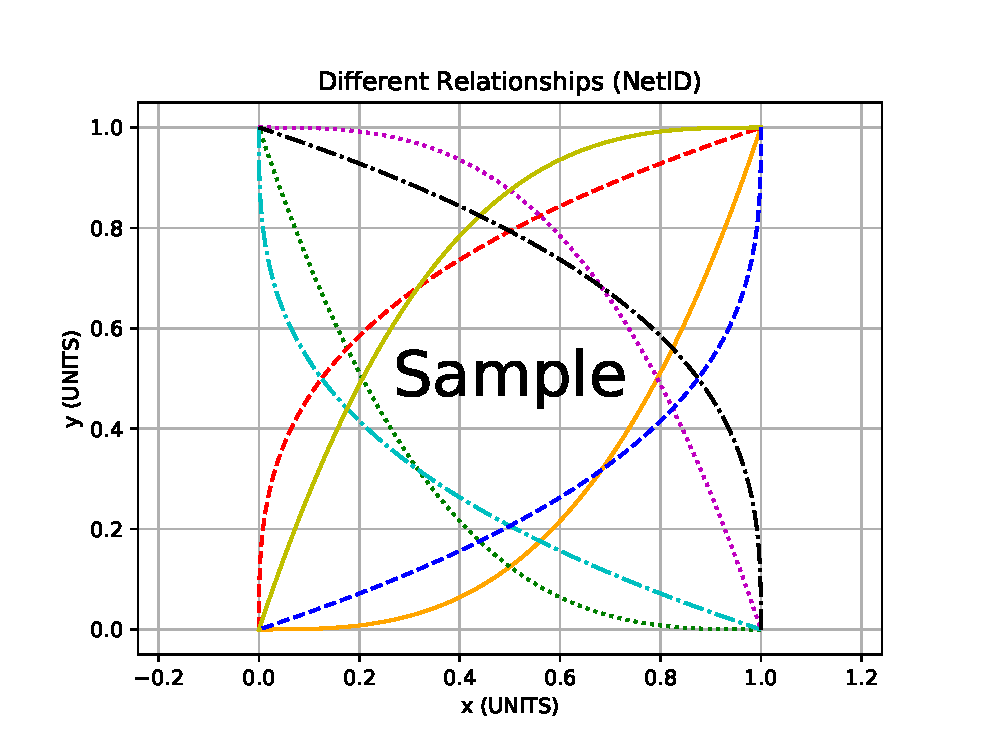
\epsfig{file=SamplePyplot.eps, width=4in} 
\caption{Sample figure.}
\end{center}
\end{figure}
\pagebreak

%%% Everything in this section is done; make sure you 
%%% understand how it works in general
%%% Note that line returns are optional
\addcontentsline{toc}{section}{References}
\begin{thebibliography}{9}
\bibitem{Rizzoni}
  Rizzoni, Georgio,
  {\it Principles and Applications of Electrical Engineering}.
  McGraw-Hill, New York,
  5th Edition,
  2007.
\bibitem{Hibbeler}
Hibbeler, R. C.,
{\it Mechanics of Materials}.
Pearson Prentice Hall, Upper Saddle River, NJ, 8th Edition, 2011.
\bibitem{Kreyszig}
Kreyszig, Erwin,
{\it Advanced Engineering Mathematics}.
John Wiley \& Sons, New York, 8th Edition, 1999.
\bibitem{Ott}
Ott, Edward,
{\it Chaos in Dynamical Systems}.
Cambridge University Press, Cambridge, UK, 1st Edition, 1993.
\bibitem{Ostwald}
Wikipedia, 
{\it Ostwald process} (http://en.wikipedia.org/wiki/Ostwald$\_$process).
Online; accessed 19-Aug-2012.
\end{thebibliography}

\end{document}
